\section{Introduction}






There are some prediction tasks where the output labels are discrete and are periodic. For example, consider the problem of pose estimation. Although pose can be a continuous variable, in practice, it is often discretized $e.g.$, in 5-degree intervals. Because of the periodic nature of pose, a 355-degree label is closer to 0-degree label than the 10-degree label. Thus it is important to consider the periodic and discrete nature of the pose classification problem.


In previous literature, pose estimation is often cast as a multi-class classification problem \cite{raza2018appearance}, a metric regression problem \cite{prokudin2018deep}, or a mixture of both \cite{mahendran2018mixed}.

In a multi-class classification formulation using the cross-entropy (CE) loss, the class labels are assumed to be independent from each other \cite{raza2018appearance,liu2019research,liu2019feature}. Therefore, the inter-class similarity is not properly exploited. For instance, in Fig. \ref{fig:1}, we would prefer the predicted probability distribution to be concentrated near the ground truth class, while the CE loss does not encourage that.

On the other hand, metric regression methods treat the pose as a continuous numerical value \cite{liu2017adaptive,liu2018adaptive,liu2019hard}, although the label of pose itself is discrete. As manifested in \cite{liu2018ordinal,liu2019unimodala,liu2019unimodalb}, learning a regression model using discrete labels will cause over-fitting and exhibit similar or inferior performance compared with classification.

Recent works either use a joint classification and regression loss \cite{mahendran2018mixed} or divide a circle into several sectors with a coarse classification that ignores the periodicity, and then applying regression networks to each sector independently as an ordinal regression problem \cite{hara2017designing}. Unfortunately, none of them fundamentally address the limitations of CE or regression loss in angular data. 




\begin{figure}[t]
\centering
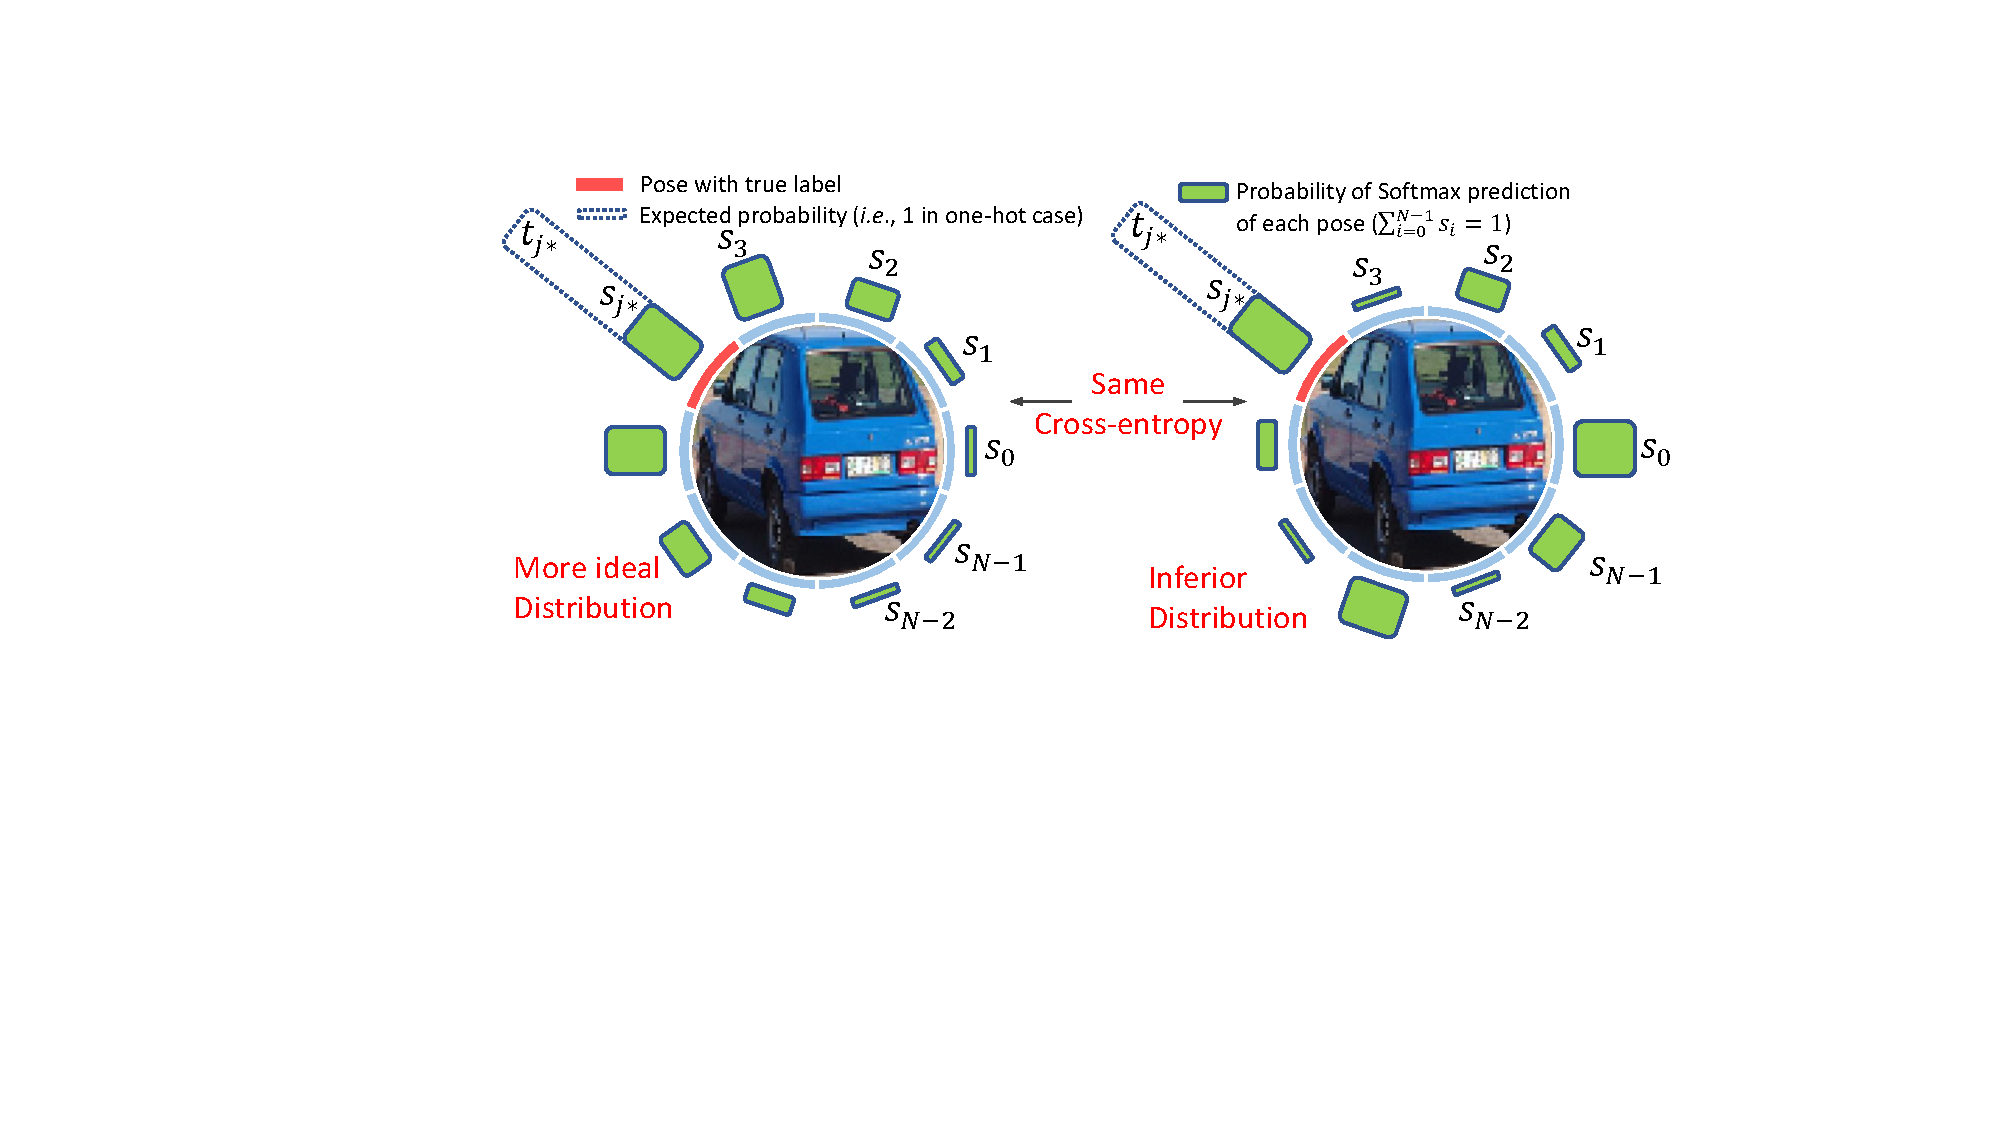
\includegraphics[width=8.3cm]{fig//figx.pdf}\\
\caption{The limitation of CE loss for pose estimation. The ground truth direction of the car is $t_j \ast$. Two possible softmax predictions (green bar) of the pose estimator have the same probability at $t_j \ast$ position. Therefore, both predicted distributions have the same CE loss. However, the left prediction is preferable to the right, since we desire the predicted probability distribution to be larger and closer to the ground truth class.}\label{fig:1} 
\end{figure}



In this work, we employ the Wasserstein loss as an alternative for empirical risk minimization. The $1^{st}$ Wasserstein distance is defined as the cost of optimal transport for moving the mass in one distribution to match the target distribution \cite{rubner2000earth,ruschendorf1985wasserstein}. Specifically, we measure the Wasserstein distance between a softmax prediction and its target label, both of which are normalized as histograms. By defining the ground metric as class similarity, we can measure prediction performance in a way that is sensitive to correlations between the classes. 




The ground metric can be predefined when the similarity structure is known a priori to incorporate the inter-class correlation, $e.g.,$ the arc length for the pose. We further extend the arc length to its increasing function from an optimization perspective. The exact Wasserstein distance in one-hot target label setting can be formulated as a soft-attention scheme of all prediction probabilities and be rapidly computed. We also propose to learn the optimal ground metric following alternative optimization.  

Another challenge of pose estimation comes from low image quality ($e.g.,$ blurry, low resolution) and the consequent noisy labels. This requires 1) modeling the noise for robust training \cite{liu2019unimodala,liu2019unimodalb} and 2) quantifying the uncertainty of predictions in testing phase \cite{prokudin2018deep}.


Wrongly annotated targets may bias the training process \cite{szegedy2016rethinking,belagiannis2015robust}. We instigate two types of noise. The outlier noise corresponds to one training sample being very distant from others by random error and can be modeled by a uniform distribution \cite{szegedy2016rethinking}. We notice that the pose data is more likely to have inlier noise where the labels are wrongly annotated as the near angles and propose to model it using a unimodal distribution. Our solution is to construct a conservative target distribution by smoothing the one-hot label using a wrapped uniform-unimodal mixture model.

Unlike the one-hot setting, the conservative target distribution makes the computation of Wasserstein distance more advanced because of the numerous possible transportation plans. The $\mathcal{O}(N^3)$ computational complexity for $N$ classes has long been a stumbling block in using Wasserstein distance for large-scale applications. Instead of only obtaining its approximate solution using a $\mathcal{O}(N^2)$ complexity algorithm  \cite{cuturi2013sinkhorn}, 
we systematically analyze the fast closed-form computation of Wasserstein distance for our conservative label when our ground metric is a linear, convex, or concave increasing function $w.r.t.$ the arc length. The linear and convex cases can be solved with linear complexity of $\mathcal{O}(N)$. Our $exact$ solutions are significantly more efficient than the approximate baseline. 






The main contributions of this paper are summarized as

$\bullet$ We cast the pose estimation as a Wasserstein training problem. The inter-class relationship of angular data is explicitly incorporated as prior information in our ground metric which can be either pre-defined (a function $w.r.t.$ arc length) or adaptively learned with alternative optimization. 


$\bullet$ We model the inlier and outlier error of pose data using a wrapped discrete unimodal-uniform mixture distribution, and regularize the target confidence by transforming one-hot label to conservative target label.


$\bullet$ For either one-hot or conservative target label, we systematically conclude the possible fast closed-form solution when a non-negative linear, convex or concave increasing mapping function is applied in ground metric.  

We empirically validate the effectiveness and generality of the proposed method on multiple challenging benchmarks and achieve the state-of-the-art performance.

